\documentclass[12pt]{article} 

\usepackage{geometry}

\geometry{a4paper}

\usepackage[utf8]{inputenc}
\usepackage[spanish]{babel}
\usepackage{graphicx}
\usepackage{url}
\usepackage{mathtools}
\usepackage{hyperref}
\usepackage{xcolor}
\usepackage{epigraph}
\usepackage{float} 
\usepackage{wrapfig}
\usepackage{lipsum}
\usepackage{algorithm}
\usepackage[noend]{algpseudocode}
\usepackage{multirow}
\usepackage{array}

% Redefinir palabras clave en español
\algrenewcommand\algorithmicprocedure{\textbf{Procedimiento}}
\algrenewcommand\algorithmicend{\textbf{fin}}
\algrenewcommand\algorithmicif{\textbf{si}}
\algrenewcommand\algorithmicelse{\textbf{sino}}
\algrenewcommand\algorithmicthen{\textbf{entonces}}
\algrenewcommand\algorithmicfor{\textbf{para}}
\algrenewcommand\algorithmicdo{\textbf{hacer}}
\algrenewcommand\algorithmicreturn{\textbf{devolver}}

\floatname{algorithm}{Algoritmo}

\linespread{1.2}
\hypersetup{
    colorlinks,
    linkcolor={gray!50!black},
    citecolor={blue!50!black},
    urlcolor={blue!80!black}
}

\graphicspath{ {./images/} }

\makeatletter
\renewcommand{\ALG@beginalgorithmic}{\small}
\makeatother

\newcolumntype{C}[1]{>{\centering\arraybackslash}p{#1}}

\begin{document}

%----------------------------------------------------------------------------------------
%	TITLE PAGE
%----------------------------------------------------------------------------------------

\begin{titlepage}
\title{Machine Learning aplicado a las CCSS}
\newcommand{\HRule}{\rule{\linewidth}{0.5mm}} % Defines a new command for the horizontal lines, change thickness here

\center % Center everything on the page


\includegraphics[scale=0.25]{uned_emp}\\[.5cm]

\textsc{\large \bfseries GRADO EN ECONOMÍA}\\[.5cm] % Name of your university/college

\vspace{25mm}
\textsc{\Large Machine Learning aplicado a las CCSS}\\[1.2cm]
\HRule \\[0.4cm]
{ \LARGE \bfseries Predicción del PIB con Modelos de ML}\\[0.5cm] % Title of your document
\HRule \\[.5cm]
\vspace{10mm}

\vspace{10mm}

{\large 10 de septiembre de 2023}\\[4cm] 

\raggedright

{\large \textbf{Autor:} Gustavo Eduardo Vargas Núñez}\\[.3cm]
{\large \textbf{Profesor:} Alberto Muñóz Cabanes}\\[.3cm]
\vspace{5mm}

\end{titlepage}

%----------------------------------------------------------------------------------------
%	TABLE OF CONTENTS
%----------------------------------------------------------------------------------------

\tableofcontents

\newpage

%----------------------------------------------------------------------------------------
%	ABSTRACT
%----------------------------------------------------------------------------------------

% \begin{abstract}
% Vamos a usar método de Machine Learning basados en árboles para predecir 

% \end{abstract}

% \vfill

%----------------------------------------------------------------------------------------
%	INTRODUCCIÓN
%----------------------------------------------------------------------------------------

\section{Introducción}

El Producto Interno Bruto (PIB) per cápita es uno de los indicadores económicos más referenciados a nivel mundial. Al representar el valor promedio de la producción de bienes y servicios que corresponde a cada habitante de un país en un periodo determinado, este indicador nos proporciona una instantánea de la salud económica de una nación y su capacidad para proporcionar prosperidad a su población. Considerar el PIB per cápita es esencial, ya que no sólo refleja la magnitud de la economía en sí, sino también hasta qué punto los beneficios de esta economía están siendo compartidos entre los ciudadanos. Su estudio nos permite comprender las disparidades económicas entre naciones y regiones, y evaluar la eficacia de las políticas económicas. Asimismo, es una herramienta invaluable para analizar tendencias a lo largo del tiempo, identificar desafíos y proyectar escenarios futuros.

En el presente estudio, vamos a predecir el Producto Interno Bruto (PIB) per cápita mediante la aplicación de técnicas avanzadas de Machine Learning. En específico, se han seleccionado modelos basados en árboles, incluyendo Árboles de Decisión, Random Forest, XGBoost y Light GBM, con la intención de explorar y evaluar sus capacidades predictivas en contextos económicos.

El estudio aborda dos enfoques diferentes. El primero se centra en la predicción de la serie absoluta del PIB per cápita, mientras que el segundo analiza la predicción de las variaciones anuales de dicho indicador. Este doble enfoque nos permitirá saber si alguno de los dos presenta una mayor susceptibilidad a ser predicho con precisión por los modelos seleccionados.

Un componente esencial de nuestro análisis radica en la interpretación de los factores o variables que más influyen en las predicciones. Afortunadamente, los modelos basados en árboles ofrecen una ventaja significativa en este aspecto, ya que incorporan el método denominado \textit{feature importance}. Mediante este método, es posible identificar las variables según su grado de relevancia en la predicción del PIB per cápita. Esta evaluación no sólo proporciona una visión detallada sobre los determinantes subyacentes del PIB per cápita según los modelos, sino que también puede ser instrumental en la formulación de políticas y estrategias económicas basadas en datos.

\section{Datos}

El PIB per cápita es una medida económica que se obtiene al dividir el Producto Interno Bruto (PIB) total de un país por su población total. Es utilizado frecuentemente como un indicador de la renta media de los habitantes de una nación y puede expresarse en términos nominales o reales.

En el contexto de esta investigación, se ha recurrido a la base de datos del proyecto Maddison, una fuente reconocida por su meticulosa recopilación y análisis de series temporales a largo plazo del PIB. En específico, los datos seleccionados hacen referencia al PIB real per cápita, y están ajustados a dólares constantes del año 2011. Esta elección garantiza una comparación homogénea y ajustada por inflación a lo largo del periodo de estudio, permitiendo así un análisis más preciso y fundamentado sobre las tendencias y comportamientos del PIB per cápita a nivel global.	Usaremos los datos disponibles para España a partir de 1850 hasta 2018, como se puede ver en la Figura 1.

\begin{center}
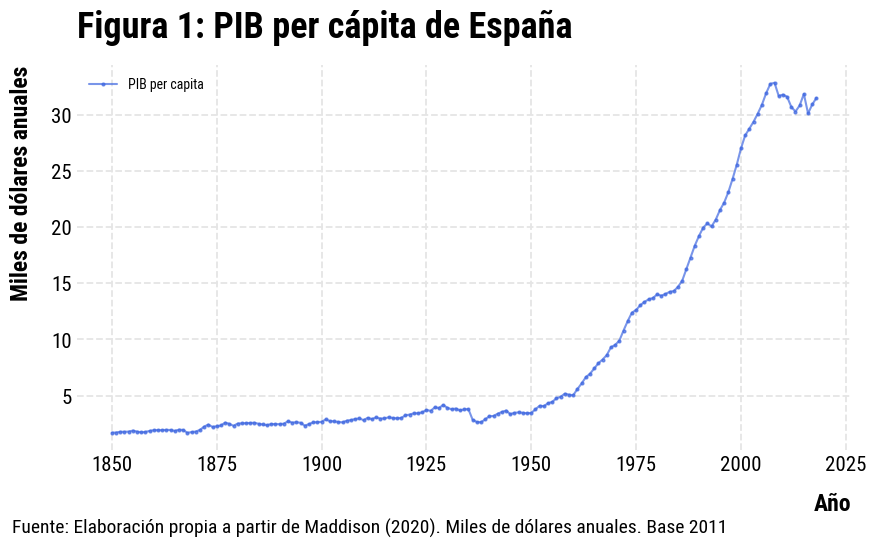
\includegraphics[scale=0.65]{fig_1_pibpc}
\end{center}

En una segunda parte del estudio utilizaremos los rendimientos interanuales correspondientes a los años de estudio. Se pueden ver en la Figura 2.

\begin{center}
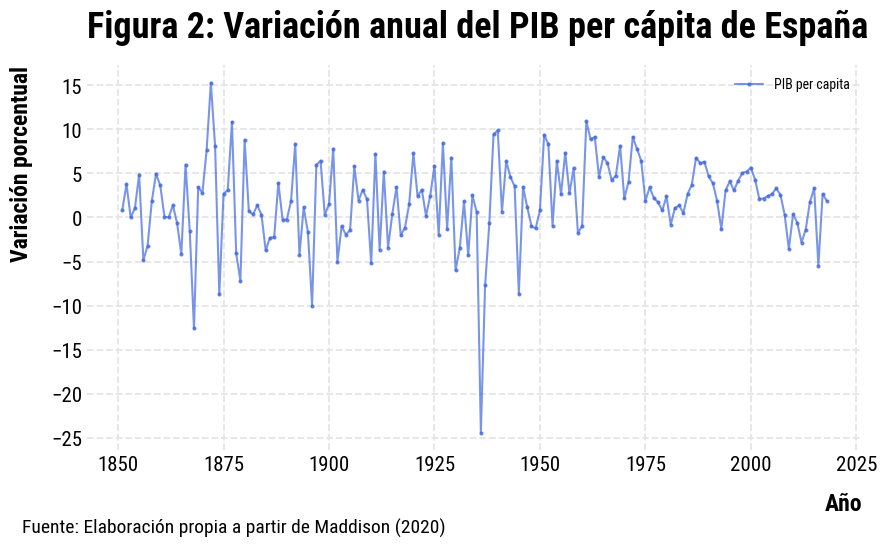
\includegraphics[scale=0.65]{fig_2_varpibpc}
\end{center}


\section{Metodología}

Se adopta un enfoque de procesamiento de datos orientado a la estructuración de un problema de regresión. Con este propósito, se segmentarán los datos en ventanas temporales de 8 años. De cada ventana, se emplearán los datos correspondientes a los primeros 7 años para prever el valor del octavo año. Los algoritmos seleccionados para este estudio están diseñados para minimizar el error cuadrático.


Es esencial mencionar que basar la evaluación del modelo en el error calculado sobre los datos de entrenamiento puede ser inapropiado. Por ende, es necesario dividir el conjunto de datos en otros dos: \textit{datos de entrenamiento} y \textit{datos de test}. A fin de evitar solapamientos y garantizar la integridad de la información temporal, se eliminarán las 7 filas que se encuentran entre dichos dos subconjuntos. Este procedimiento y su lógica se ilustran en la Figura 3.

\begin{figure}[H]
  \makebox[\textwidth][c]{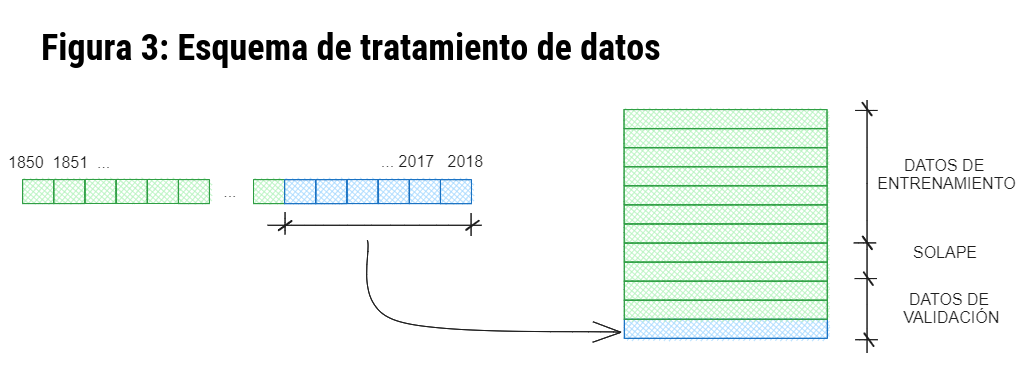
\includegraphics[width=1.2\textwidth]{fig_3_schema}}
\end{figure}

\subsection{Algoritmos}

Los algoritmos que vamos a utilizar son algoritmos basados en árboles. Se ha decidido hacerlo así por su mejor capacidad predictiva con pequeñas base de datos, además de una mejor interpretabilidad en el \textit{porqué} de sus predicciones.



Para este estudio, se ha optado por emplear algoritmos basados en árboles. Esta elección responde a la eficacia demostrada de dichos algoritmos con conjuntos de datos de dimensiones reducidas, así como a la interpretabilidad con la que permiten entender las razones de sus predicciones mediante el método de \textit{feature importance}. Ésto contrasta con los algoritmos de \textit{aprendizaje profundo}, donde la interpretabilidad es, a priori, nula.

\subsubsection{Árboles de Decisión}

Un Árbol de Decisión para regresión es una herramienta de aprendizaje supervisado que predice valores continuos en lugar de etiquetas de clase. La estructura de un árbol de decisión consta de nodos, ramas y hojas. Cada nodo representa una característica o atributo del conjunto de datos, cada rama representa una decisión basada en un valor de ese atributo y cada hoja es el resultado, que en el caso de la regresión es un valor numérico.

El proceso de construcción de un árbol de regresión implica seleccionar el atributo que proporciona la mejor división en función de un criterio determinado, generalmente la reducción de varianza. Una vez que se selecciona un atributo para un nodo, el conjunto de datos se divide en subconjuntos según los valores de ese atributo. Este proceso se repite de manera recursiva para cada subconjunto hasta que se alcanza un criterio de parada, como una profundidad máxima del árbol o un número mínimo de puntos de datos en un nodo.

\begin{algorithm}
\caption{Árbol de Decisión para Regresión}
\begin{algorithmic}
\Procedure{ÁrbolDeDecisiónRegresión}{Datos, Criterio}
    \If{todos los ejemplos en Datos tienen el mismo valor}
        \State \Return valor promedio
    \EndIf
    \If{Lista de Atributos está vacía o se cumple otro criterio de parada}
        \State \Return valor promedio de los valores en Datos
    \EndIf
    \State MejorAtributo $\leftarrow$ seleccionarMejorAtributo(Datos, Criterio)
    \State Árbol $\leftarrow$ nuevo nodo con MejorAtributo
    \For{cada valor v posible de MejorAtributo}
        \State Datos\_v $\leftarrow$ ejemplos en Datos donde MejorAtributo = v
        \If{Datos\_v está vacío}
            \State añadir una rama a Árbol con etiqueta v
            \State nodo hoja con valor promedio en Datos
        \Else
            \State añadir rama a Árbol con etiqueta v
            \State \Call{ÁrbolDeDecisiónRegresión}{Datos\_v, Criterio}
        \EndIf
    \EndFor
    \Return Árbol
\EndProcedure
\end{algorithmic}
\end{algorithm}



\subsubsection{Random Forest}

Random Forest es un algoritmo que combina múltiples árboles de decisión para construir un modelo más robusto y preciso. Se basa en dos técnicas principales: bagging y feature randomness.

\begin{itemize}
  \item Bagging: Para cada árbol del bosque, se toma una muestra con reemplazo (conocida como muestra bootstrap) del conjunto de datos original. Esto significa que algunos ejemplos pueden ser seleccionados más de una vez y otros no ser seleccionados en absoluto para un árbol en particular.
  \item Feature randomness: Al construir cada árbol, en lugar de buscar la mejor característica para dividir en cada nodo, se selecciona un subconjunto aleatorio de características y luego se busca la mejor característica para dividir solo dentro de ese subconjunto.
\end{itemize}

Una vez entrenado el modelo, para realizar una predicción, se ejecuta el ejemplo a través de todos los árboles en el bosque y se toma el promedio de sus predicciones para obtener la predicción final del modelo.

\begin{algorithm}
\caption{Random Forest para Regresión}
\begin{algorithmic}
\Procedure{RandomForestRegresión}{Datos, n\_árboles, n\_características}
    \State Inicializar lista vacía Árboles
    \For{\(i = 1\) hasta n\_árboles}
        \State Muestra\_bootstrap $\leftarrow$ generarMuestraBootstrap(Datos)
        \State Árbol $\leftarrow$ construirÁrbolDecisión(Muestra\_bootstrap, n\_características)
        \State Añadir Árbol a Árboles
    \EndFor
    \Procedure{predecir}{ejemplo}
        \State predicciones $\leftarrow$ [Árbol.predecir(ejemplo) para Árbol en Árboles]
        \State \Return promedio(predicciones)
    \EndProcedure
\EndProcedure
\end{algorithmic}
\end{algorithm}


\subsubsection{XGBoost}

XGBoost, que proviene de 'Extreme Gradient Boosting', es un algoritmo de aprendizaje supervisado que utiliza un enfoque de boosting para construir un conjunto de árboles de decisión. El objetivo principal de XGBoost es optimizar un conjunto de modelos débiles, generalmente árboles de decisión, de manera aditiva y secuencial. Estos son algunos aspectos clave de su funcionamiento:

\begin{itemize}
  \item Función de Pérdida: La base del método XGBoost es minimizar una función de pérdida. En el caso de la regresión, la función de pérdida más comúnmente utilizada es la diferencia cuadrada entre las predicciones y los valores verdaderos. Sin embargo, XGBoost puede adaptarse a diferentes funciones de pérdida y se puede utilizar para tareas de clasificación y ranking, además de la regresión.
  \item Boosting: XGBoost utiliza un enfoque de boosting, lo que significa que construye árboles de manera secuencial, donde cada árbol corrige los errores del anterior. A diferencia de otros algoritmos de boosting, XGBoost también tiene en cuenta un término de regularización en su función objetivo, lo que ayuda a evitar el sobreajuste.
  \item Descenso de Gradiente: A medida que construye cada árbol, XGBoost utiliza el descenso de gradiente para minimizar el error entre las predicciones actuales y los valores reales. Específicamente, calcula el gradiente (primera derivada) y el hessiano (segunda derivada) de la función de pérdida con respecto a las predicciones del modelo anterior para guiar la construcción del siguiente árbol.
  \item Regularización: XGBoost incluye términos de regularización en su función objetivo, lo que tiene el efecto de penalizar modelos más complejos y ayudar a prevenir el sobreajuste. Esta regularización se aplica tanto a la estructura de los árboles individuales (como la profundidad del árbol) como a las ponderaciones de las predicciones de los árboles.
  \item Optimización de la Estructura del Árbol: XGBoost utiliza un criterio llamado 'ganancia' para determinar las divisiones en cada árbol. La ganancia es la reducción en la función de pérdida que se obtiene al realizar una división en particular. Al seleccionar las divisiones que producen la máxima ganancia, XGBoost construye árboles que son óptimos en términos de reducir la función de pérdida.
  \item Paralelización: Aunque el proceso de boosting es inherentemente secuencial (cada árbol debe construirse después del anterior), XGBoost está diseñado para paralelizar la construcción de los árboles individuales. Esto significa que puede construir un árbol más rápidamente al utilizar múltiples núcleos de CPU.
  \item Pruning: A diferencia de la mayoría de los algoritmos de árboles que utilizan una estrategia de 'pruning' basada en la profundidad (limitan la profundidad máxima de un árbol), XGBoost utiliza 'depth-first pruning'. Es decir, permite que un árbol crezca en profundidad hasta que cumpla con ciertos criterios, y luego poda el árbol retrocediendo y eliminando ramas que aportan poco valor.
\end{itemize}


\begin{algorithm}
\caption{XGBoost para Regresión}
\begin{algorithmic}
\Procedure{XGBoostRegresión}{Datos, n\_árboles, tasa\_aprendizaje, regularización}
    \State Inicializar modelo con predicciones constantes (p. ej., promedio de los objetivos)
    \For{\(i = 1\) hasta n\_árboles}
        \State Calcular gradientes y hessianos de la función de pérdida
        \State Construir árbol usando gradientes y hessianos
        \State Actualizar modelo sumando tasa\_aprendizaje $\times$ predicciones del nuevo árbol
    \EndFor
    \Procedure{predecir}{ejemplo}
        \State Sumar predicciones de todos los árboles para el ejemplo 
        \State \Return Predicción final
    \EndProcedure
\EndProcedure
\end{algorithmic}
\end{algorithm}




\subsubsection{LightGBM}

LightGBM, acrónimo de 'Light Gradient Boosting Machine', es un framework de boosting optimizado para conjuntos de datos grandes y altamente dimensional. A continuación, se presentan características y detalles clave de su funcionamiento:

\begin{itemize}
  \item Crecimiento basado en hojas: A diferencia de otros algoritmos de boosting que construyen árboles nivel por nivel, LightGBM sigue una estrategia de crecimiento basada en hojas. Mientras que los enfoques tradicionales crecen el árbol de manera uniforme, LightGBM divide la hoja que aporta la máxima reducción en la función de pérdida, permitiendo un aprendizaje más dirigido y, a menudo, un error menor.
  \item Optimización para Conjuntos de Datos Grandes: LightGBM utiliza histogramas para agrupar características continuas en intervalos discretos. Estos histogramas reducen significativamente el número de divisiones a considerar y, por lo tanto, aceleran el proceso de formación del árbol.
  \item Manejo de Características Categóricas: LightGBM puede manejar características categóricas sin la necesidad de transformaciones previas. A diferencia de los enfoques tradicionales que utilizan codificación one-hot, LightGBM busca la división óptima de las características categóricas basada en la función de pérdida.
  \item Regularización: Para evitar el sobreajuste, LightGBM incorpora términos de regularización en su función objetivo. Estos términos pueden aplicarse tanto a las estructuras de los árboles (por ejemplo, controlando la profundidad o el número de hojas) como a las ponderaciones de las predicciones.
  \item Técnicas de Boosting: Al igual que otros métodos de boosting, LightGBM construye árboles de forma iterativa, donde cada árbol se construye para corregir los errores del conjunto de árboles anterior.
  \item Uso Eficiente de la Memoria: Las optimizaciones de LightGBM, como la creación de histogramas, permiten que el algoritmo utilice menos memoria en comparación con otros métodos de boosting.
  \item Paralelización y Escalabilidad: LightGBM está diseñado para escalar a lo largo de grandes conjuntos de datos y distribuirse en múltiples máquinas. Utiliza técnicas como la construcción de árboles basada en características para paralelizar el entrenamiento, lo que mejora la eficiencia en conjuntos de datos con un alto número de características.
  \item Soporte para Valores Perdidos: LightGBM tiene incorporado el manejo de valores perdidos. Durante el proceso de construcción del árbol, determina la dirección óptima para las observaciones con valores perdidos, ya sea a la división izquierda o derecha.
\end{itemize}


\begin{algorithm}
\caption{LightGBM para Regresión}
\begin{algorithmic}[1]
\Procedure{LightGBMRegresión}{Datos, n\_árboles, tasa\_aprendizaje}
    \State Inicializar modelo con predicciones constantes
    \For{\(i = 1\) hasta n\_árboles}
        \State Calcular gradientes de la función de pérdida
        \State Construir árbol utilizando estrategia de crecimiento basada en hojas
        \State Actualizar modelo sumando tasa\_aprendizaje $\times$ predicciones del nuevo árbol
    \EndFor
    \Procedure{predecir}{ejemplo}
        \State Sumar predicciones de todos los árboles para el ejemplo
        \State \Return Predicción final
    \EndProcedure
\EndProcedure
\end{algorithmic}
\end{algorithm}
 
\subsection{Experimentación}



\subsubsection{Cross Validation}

Cross Validation, o validación cruzada, es una técnica de evaluación de modelos en el aprendizaje automático que busca estimar el rendimiento de un modelo en datos no vistos. La idea central es dividir el conjunto de datos original en "k" subconjuntos (o "folds"). En cada iteración, se utiliza un subconjunto como datos de validación y los "k-1" subconjuntos restantes como datos de entrenamiento.

El proceso se repite "k" veces, rotando el subconjunto de validación en cada iteración. Al final de las "k" iteraciones, se obtiene una serie de métricas de rendimiento, como el error, para cada fold. Estas métricas se promedian para obtener una estimación más robusta y menos sesgada del rendimiento del modelo en comparación con usar una única división de entrenamiento y validación.


\subsubsection{Grid Search}

Grid Search es una técnica utilizada en el aprendizaje automático para optimizar hiperparámetros. Funciona definiendo un conjunto de valores posibles para cada hiperparámetro y luego evaluando todas las posibles combinaciones de estos valores. Para cada combinación, se entrena un modelo sobre un conjunto de datos de entrenamiento y se valida su rendimiento en un conjunto separado.

Después de examinar todas las combinaciones, se selecciona la que haya producido el mejor rendimiento en el conjunto de validación. Si bien Grid Search es exhaustivo y puede identificar una combinación óptima, tiene un alto coste computacional, especialmente cuando el espacio de búsqueda de hiperparámetros es grande o el modelo es computacionalmente intensivo.

\section{Resultados}

Podemos ver los resultados de los experimentos en el Cuadro 1. Los modelos de Machine Learning intentan aproximarse a la distribución de los datos con la que han sido entrenados, de ahí que sea necesario tener datos de test para poder tener una métrica significa del rendimiento de nuestro modelo.

Como vemos, tanto el modelo de Árboles de Decisión como XGBoost tienen un error en entrenamiento menor que en test, lo que es normal. Lo significativo pasa en los otros dos modelos, Random Forest y Light GBM, donde el error en test es menor que en entrenamiento, especialmente en el caso del Light GBM.

\begin{table}[H]
\centering
\caption{Resultados de los Experimentos}
\begin{tabular}{l C{2.5cm} C{2.5cm}}
\multirow{2}{*}{}     & \multicolumn{2}{c}{\textbf{Error Cuadrático Medio}}              \\ \cline{2-3} 
                      & \textbf{Train} & \textbf{Test} \\ \hline
Decision Tree & 0.00122 & 0.00189 \\ \hline
Random Forest & 0.00153 & 0.00118 \\ \hline
XGBoost       & 0.00023 & 0.00124 \\ \hline
Light GBM     & 0.00216 & 0.00082 \\ \hline
\end{tabular}
\end{table}

La Figura 4 nos permite explicar el porqué de ello. Ahí vemos la variación del PIB per cápita en azul en test y la comparamos con las distintas predicciones. En el caso de Light GBM, la predicción no varía mucho, dando una curva relativamente plana. Ésto, sin embargo, es lo que le permite tener un error relativamente pequeño, ya que en el resto de casos las predicciones se separan mucho más de los valores reales.

\begin{figure}[H]
  \makebox[\textwidth][c]{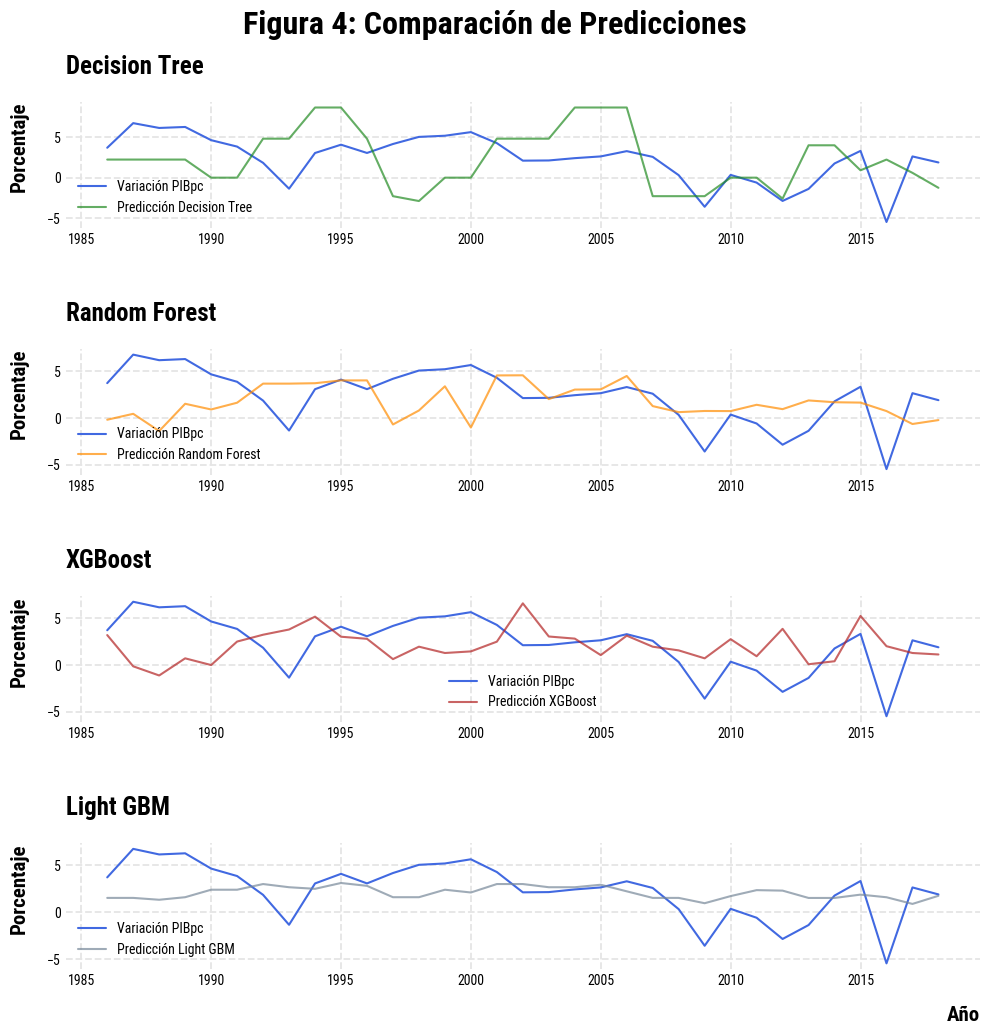
\includegraphics[width=1\textwidth]{fig_4_comparacion.png}}
\end{figure}
 

\section{Conclusiones}

Predecir una serie temporal nunca es tarea fácil. En nuestro caso, el problema se ha visto agravado por la escasez de datos históricos que tenemos para la variable que nos interesa, el PIB per cápita. Sin embargo, hemos visto que estas predicciones son posibles. Hemos probado cuatro modelos, siendo el Light GBM con el que hemos obtenido las predicciones con menos error.

Posibles ampliaciones del trabajo tendrían en cuenta las siguientes líneas:
\begin{itemize}
    \item El entrenamiento podría hacerse con las series de todos los países y ver si eso ayuda a mejorar la predicción. Se podría intentar, al menos, buscar un subconjunto de países con comportamiento histórico similar y ceñir el entrenamiento a ellos.
    \item Se debería hacer una comparación con modelos autorregresivos, especialmente los tipo GARCH, para poder comparar el grado de error.
    \item Parsear los datos de la forma en la que lo hemos hecho convierte el problema en uno de regresión sobre datos tabulares. Esto permite añadir nuevas \textit{features}, con la única limitación de que dichas features deberían estar disponibles para el período estudiado.
\end{itemize}


\newpage

\begin{thebibliography}{1}

\bibitem{maddison2020}
Bolt, Jutta and J.L. Van Zanden, (2020).
\newblock {\em Maddison style estimates of the evolution of the world economy. A new 2020 update}.
\newblock Maddison Project Database.

\bibitem{adaboost}
M.A. Hambali, Y.K. Saheed, T.O. Oladele, M. D. Gbolagade.
\newblock {\em ADABOOST Ensemble Algorithms for Breast Cancer Classification}.
\newblock Journal of Advances in Computer Research. Vol. 10. No. 2, May 2019. Pages: 31-52

\bibitem{rf}
Hongquan Guo, Hoang Nguyen, Diep-Anh Vu, Xuan-Nam Bui.
\newblock {\em Forecasting mining capital cost for open-pit mining project based on artificial neural network approach}.
\newblock Resources Policy. Vol. 74, December 2021, 101474.

\bibitem{xgboost}
Chao Qin, Yunfeng Zhang, Fangxun Bao, Caiming Zhang, Peide Liu, Peipei Liu.
\newblock {\em XGBoost Optimized by Adaptative Particle Swarm Optimization for Credit Scoring}.
\newblock Mathematical Problems in Engineering. Vol. 2021. Article ID 6655510.

\bibitem{lightgbm}
N. Dunbray, R. Rane, S. Nimje, J. Katade and S. Mavale.
\newblock {\em A Novel Prediction Model for Diabetes Detection Using Gridsearch and A Voting Classifier between Lightgbm and KNN}.
\newblock IEEE. 2021 2nd Global Conference for Advancement in Technology (GCAT), Bangalore, India, 2021, pp. 1-7

\end{thebibliography}
\end{document}